\documentclass[a4paper,12pt]{article}
\usepackage{ecography}
\usepackage{lmodern}
\usepackage{amsmath}
\usepackage{xfrac}

 \renewcommand{\familydefault}{\sfdefault}


\title{A Recipe for Scavenging - the natural history of a behaviour}
\running{Scavenging in vertebrates}

\author{Adam Kane, Kevin Healy, Thomas Guillerme, Graeme Ruxton, \& Andrew Jackson.}

\affiliations{
\item A. Kane (\url{adam.kane@ucc.ie}), University College Cork, Cooperage Building, School of Biological Earth and Environmental Sciences, Cork, Ireland.
\item K. Healy and A. Jackson, Trinity College Dublin, Department of Zoology, School of Natural Sciences, Dublin Ireland.
\item T. Guillerme, Imperial College London, Silwood Park Campus, Department of Life Sciences, Buckhurst Road, Ascot SL5 7PY, United Kingdom.
\item G. Ruxton, School of Biology, Sir Harold Mitchell Building, Greenside Place, St Andrews, KY16 9TH, United Kingdom.
}

\nwords{9999}


\begin{document}

\maketitle


\begin{abstract}
Despite its prevalence cavenging is a difficult behaviour to observe in modern day carnivores. Yet, there are certain intrinsic and environmental features of a speices that push it towards a scavenging lifestlye. Chief among these are low-cost locomotion, high detection distances, effective carrion processing and a carrion producing environment. 
\end{abstract}

\newpage


\section*{Introduction}
%TG: it might be better to reorganise the intro as:
%§1 - scavenging is understudied because it's hard to say who's a scavenger
%§2 - it's even more problematic in the fossil record but people have tried some indirect approaches
%§3 - good thing is that we can apply these indirect approaches to extant systems
%§4 - in this review we discuss some stuff.
%TG: or something along these lines, obviously flexible!
Historically, scavengers have not been viewed as the most charismatic of animals.
This may go some way to explaining the gap in our knowledge of the prevalence of this behaviour.
Consider Professor Sanborn Tenney writing in 1877 for The American Naturalist who had this to say about one well known group, ``prominent among the mammalian scavengers are the hyenas, the ugliest in their general appearance of all the flesh eaters."
He contrasts these with ``nobler kinds" of carnivores such as lions and tigers \citep{tenney1877few}.
Even aside from our own subjective biases, scavenging is a difficult behaviour to detect after the fact.
Without catching a carnivore in the act of killing we are left to infer how the prey was killed.
Some simple heuristics can inform us, for instance, in cases where the prey item was simply too large to have been killed by the ostensible predator \citep{pobiner2008paleoecological}.
But clearly, a scavenger doesn’t only feed on animals too big for it to have hunted.
The obvious lack of direct behavioural data compounds the difficulty of discerning scavenging among extinct forms.
Indeed, a single species of dinosaur notwithstanding, a synthesis describing the natural history of scavengers is absent from the literature.
Fortunately, research on scavenging is on the rise \citep{manga2006vulture}.
As a result, we are now beginning to realise the extent of this behaviour such that, ``in some ecosystems, vertebrates have been documented to assimilate as much as 90\% of the available carrion" \citep{beasley2015vertebrates}.
Even Tenney’s noble big cats are now known to take in a significant portion of carrion in their diet where some lion populations get over 50\% of their meat from carcasses.
By recognising the difficulty in directly observing scavenging, a suite of methods have been used to discern the most suitable morphologies, physiologies and environments for a scavenging lifestyle to prosper.
Here we chart the natural history of scavenging by looking at the potential for the behaviour in dominant vertebrate groups.
%It is our aim in this review to employ these methods to gain an understanding of scavengers past and present.

\subsection*{The Difficulty of Scavenging} %KH: Make that the template for all the next sections
The chief hurdle to scavenging is finding a sufficient quantity of food, the occurence of which is difficult to predict in space and time. Thus, any animal existing as a scavenger must minimise its locomotory costs and maximise its detection capabilities \citep{ruxton2004obligate}.
Once found, the scavenger has to process the carrion and overcome the agents of decay produced by the action of microorganisms on the carcass \citep{ruxton2014fruit}. 
The habitat must also be productive enough to sustain an animal biomass that will eventually produce carcasses.
We can draw on the image of a scavenger moving through its environment, searching for food and trying to process it efficiently as we explore the prevalence of this behaviour through time. 
% The idea of scrounging from predator kills is undermined by studies showing that in the  majority of ecosystems more animals die from disease and starvation than predation \citep{benbow2015introduction}.

\begin{figure}[!htbp]
\centering
   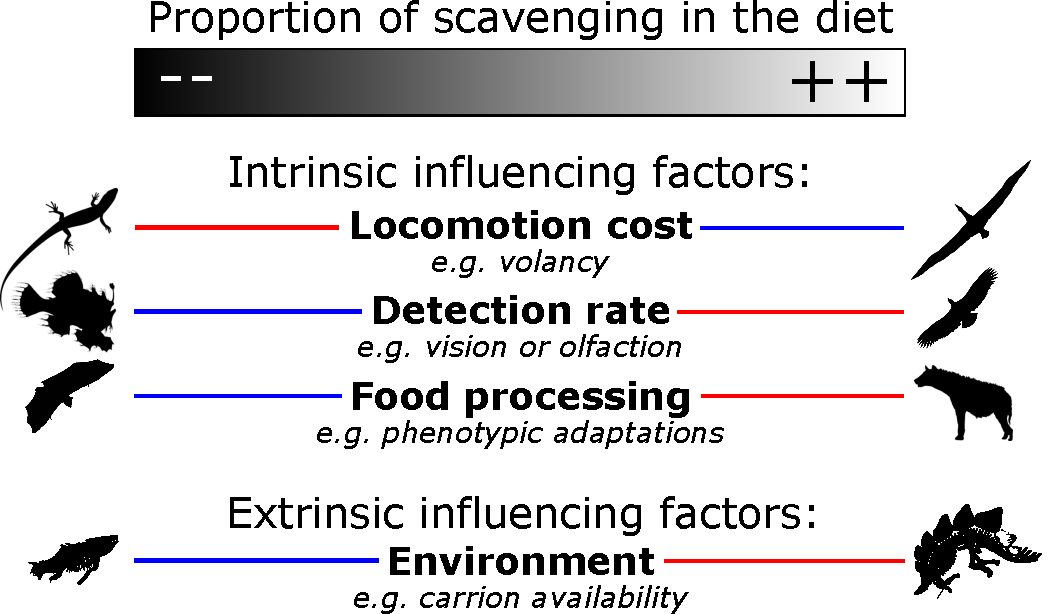
\includegraphics[width=1\textwidth]{Summary_figure/Summary_figure_Landscape.pdf}
\caption{Factors influencing the proportion of scavenging in a vertebrates' diet. Blue lines indicates a reduction in the factor and red lines indicates an increase.}
%TG: Probably needs some more explanations...
\label{Summary_figure}
\end{figure}


%KH: need paragraph for how do we know something is (was) a scavenger
%TG: Insert figure here: scavenging scale + four points: Locomotion/Detection/Consumption/Environment

% \section*{Aerial Scavengers}
% Vultures represent 
%These birds consist of two convergent groups, from the old and the new world and represent the only example of obligate vertebrate scavengers today.
%The families from which modern vultures arose, the Accipitridae and Cathartidae, appear during the Palaeocene (66 - 56 Mya) \citep{Jetz2012, Jarvis2014}.
%Given their unique position, they have been extensively studied to determine what adaptations they possess that allows them to so flourish in this niche.
%Underscoring their prowess are studies such as \cite{ogada2012effects} who note a three fold increase in carcass persistence times in the absence of vultures.
%As such, we can begin by exploring the adapdations and the environments of vultures to draw comparisons with other scavenging species and \textit{their} environments.

\subsection*{Locomotion}
As endotherms, mammals can sustain long bouts of energetically expensive activity. 
By contrast, modern reptiles are ectothermic, limiting their activity periods.
% a successful reptilian scavenger requires a far different set of adapations.
This is exacerbated by the sprawling gait seen in many lizards which results in Carrier's Constraint such that the animal can't move and breathe at the same time because the lateral movements impedes its lungs \citep{carrier1987evolution}.
This constraint manifests itself in aspects such as maximum sustainable speed where an equivalent mammal has a six to seven fold increase \citep{ruben1995evolution}.
To quantify this effect with a simple example we can turn to some allometric relationships relating sustainable travelling speed to body mass.
In the case of mammals and reptiles these are 1.15 $\times$ body mass (kg) \textsuperscript{0.12} and 0.23 $\times$ body mass (kg) \textsuperscript{0.12} respectively \citep{ruxton2004obligate}.
We can insert these into a foraging radius model $\sfrac{\frac{\text{duration} \times \text{speed}}{2}}{1000}$ for a 12 hour foraging day which shows that while a 10 kg reptile can range 6.5 km an equally sized mammal can range nearly 33 km \citep{Enstipp2006Energetics}. 
For a foraging scavenger, this ability translates into a greater area searched for food. 

Today, terrestrial scavenging in the mammals is probably best known in an African context where hyenas, jackals and lions all take sizable proportions of carrion in their diet.
In the spotted hyena (\textit{Crocuta crocuta}), striped hyena (\textit{Hyaena hyaena}) and brown hyena (\textit{Hyaena brunnea}) it can be over 90\% \citep{jones2015african}.
And although no contemporary terrestrial vertebrate exists as an obligate scavenger most if not all are facultative to some extent \citep{beasley2015vertebrates}.
The particular reliance of hyenas on carrion means we can use them as examples of efficient terrestrial scavengers to compare with other forms. 
In terms of locomotion, they employ a characteristic ``rocking horse gait"  which allows them to cover great distances efficiently, loping at 10 km/hr \citep{mills1989comparative,jones2015african}. 
Such long-distance travel is apparent in African wild dogs (\textit{Lycaon pictus}) and many other canids \citep{pennycuick1995radius,janis2014forelimb}. 
In contrast, big cats like leopards (\textit{Panthera pardus}) rely on ambush \citep{pennycuick1995radius}. 
This allows us to make a broad distinction between the ambush strategies of cats and the pursuit/ pounce strategies of dogs, the latter being more suited to scavenging \citep{janis2014forelimb}. 
We can (and have) use(d) these insights to compare extant terrestrial species to their prehistoric forebears given the dominance of mammalian carnviores since the Eocene 56-33.9 Million years ago (Mya) where the order split into the Caniforma and Feliforma \citep{van1987skeletal}.
To take one example, \cite{anyonge1996locomotor} found \textit{Nimravides}, a genus of sabretooth cat from the Miocence (10.3 to 5.3 M ya) were likely to have been ambush predators which would have counted against them taking a lot of carrion.  
%The order Carnivora saw its origins in the Middle Eocene  %TG: a phylo side note: the correct sentence would be the "The stem Carnivora saw its origins ... when it split into Caniforma and Feliforma." But I think we can leave it out because, god, it sounds pedantic!
% So we can trace efficient terrestrial movement by carnivores from this point on. 



Unsurprisingly, given their enduring appeal, the prevalence of scavenging has been explored in the carnivorous, theropod dinosaurs.
They were the dominant terrestrial forms for most of the Mesozoic Era (252.17 - 66 Mya) and ranged from the chicken-sized to the whale-sized, all of which were bipedal.
They are quite alien to anything we know today which restricts our ability to understand their ecology far more so than extinct mammals \citep{weishampel2004dinosauria}.
Of relevance, are the questions that still persist about their metabolism with the latest evidence suggesting they were mesothermic i.e. intermediate to ecto- and endotherms \citep{grady2014evidence}. 
We do know that they walked with the erect gait of mammals or birds rather than the sprawling gait of lizards and that they were most likely facultative scavengers \citep{weishampel2004dinosauria,depalma2013physical}. %TG: and cite "Kane et al in press" no? I think these people did some kind of work on that matter.
Taken together, this implies dinosaurs had a foraging range that fell in between that of modern terrestrial mammals and reptiles. 

Of course, tetrapod terrestrial dominance predates the evolution of the dinosaurs. %TG: I will down that "dominance" term. Maybe change the sentence to "Of course the importance of terrestrial tetrapods in ecosystems predates the evolution of the dinosaurs."
It is during the Permian (298.9 - 252.17 Mya) %, almost 300 millions years ago, %TG: Being pedantic here but Permian is just *not* 300 Mya... As a side note for the dates, I say we just use the geological epochs/periods/whatever since they are the actual precise dating of the fossil occurence (and they sound better). I suggest we just add the dates in brackets to give an indication.
that we have the earliest evidence of vertebrate scavenging where a temnospondyl amphibian fed on the carcass of \textit{Varanops}, a predatory synapsid of the time \citep{reisz2006articulated}. 
And it is with the evolution of endothermy in the therapsid-mammal lineage \citep{clarke2010temperature} that terrestrial vertebrates would have gained the ability to range widely, a vital component in seeking out carrion. 

Scavenging behaviour may have evolved on land as soon as the first terrestrial tetrapods emerged.
In fact, some of the earlier tetrapods tracks dating back to the early Middle Devonian (393.3 - 387.7 Mya) were found in intertidal environments \citep{Niedzwiedzki2009}.
These environments are isolated from marine systems twice a day leaving potential carrion unexploited by marine vertebrates.
\cite{Niedzwiedzki2009} suggest that these environments ``would thus have allowed marine ancestors of tetrapods gradually to acquire terrestrial competence while accessing a new and essentially untouched resource.''

%TG: I think it's missing a transition here: maybe something along "But moving on land as it's limitations..."
But it is in the air that we find scavengers par excellence. 
Flight is a cheaper means of locomotion than walking or running \citep{tucker1975energetic}. 
We know that many extant birds exist as facultative scavengers because storks, raptors and corvids all take substantial quantities of carrion in their diet \citep{kendall2013alternative}.
The advantage of flight can be extended further in larger species that engage in soaring instead of flapping flight, which is even cheaper still (approximately twice the basal metabolic rate) \citep{hedenstrom1993migration,spivey2014analysing}.
The benefits this confers are clear from the information we have on the enormous foraging ranges of many vultures \citep{spiegel2013factors} and seabirds \citep{thaxter2012seabird}.
In vultures we have the best known scavengers on Earth. 
These birds consist of two convergent groups, from the old and the new world where they represent the only example of obligate vertebrate scavengers today.
The families from which modern vultures arose, the Accipitridae and Cathartidae, appear during the Palaeocene \citep[66 - 56 Mya; ][]{Jetz2012, Jarvis2014}.
Yet, avian flight is far older than this and originates in the Late Jurassic (163.5-145 Mya), conincident with the fossils of \textit{Archaeopteryx lithographica} so many of these benefits would have been realised from that point on for carnivorous birds.
And vertebrate flight is much older still where pterosaurs predate bird origins by a considerable margin in the Late Triassic (235-201.3 Mya).
Scavenging in this diverse group has been hypothesied many times before \citep{witton2008reappraisal}.
Certain clades of these animals could reach enormous sizes \citep[e.g. Azhdarchids with wingspans of 11 metres; ][]{witton2010size} and, notably, look to have engaged in soaring flight \citep{witton2010size}.
%TG: this paragraph's a killer! Love it!

The only other vertebrate group capable of powered flight are the bats where scavenging has not been recorded to our knowledge.
The bat fossil record is notoriously poor owing to their fragile skeletons so we are unable to determine if extinct species were more suited to this lifestyle \citep{eiting2009global}. %TG: again, I'm not sure it's notoriously poor! It might be poor for mammalogist standards but it's definitely a way better than birds fossil records for example!
Although it does not seem that flight is the main criterion precluding them from scavenging (see below).

Aquatic scavengers have a locomotory benefit because water is a medium that is conducive to low-cost movement \citep{tucker1975energetic}. 
In fact, the cost of swimming is lower than either running or flying \citep{williams1999evolution}. 
This has led some researchers to argue for the feasability of a scavenging fish \citep{ruxton2004energetic,ruxton2005searching}. 
As with the aerial and terrestrial enviornments we have evidence of facultative scavenging among extinct aquatic species.
For example, the remains of a mosasaur and a terrestrial hadrosaur were discovered with embedded teeth from a Cretaceous shark, \textit{Squalicorax} \citep{schwimmer1997scavenging}.
As well as a likely instance of scavenging between a 4-million-year-old white shark (\textit{Carcharodon}) and mysticete whale from Peru \citep{ehret2009caught}.
Extant White sharks \textit{Carcharodon carcharias} too are known to feed on whale carcasses \citep{fallows2013white}. We might expect then that by combining an aquatic environment and an endothermic metabolism that marine mammals would prosper as scavengers. 
We know fossil pinnipeds and cetaceans from 60 Mya have transitional features indicative of their trajectory to fully aquatic species \citep{williams1999evolution}.  
But despite this movement away from land the energetic savings were negligible because the \textit{total} cost incurred by a swimming marine mammal is high \citep{williams1999evolution}. 
This is not to say that aquatic mammalian scavengers don't exist, only that their total energetic cost is similar to an equivalent terrestrial mammal. 
%\cite{williams1999evolution} notes, ``free-ranging animals must contend with the total energetic expenditure associated with supporting basic biological functions as well as with moving the body and appendages through the environment."

\subsection*{Detection}
It would be pointless to have incredible ranging abilites and not have the sensory architecture to benefit from it.
If we came at this from a position of complete ignorance we would predict scavengers to have well-developed senses and indeed this is what we find. 
A simplification of terrestrial, vertebrate scavengers in sensory terms is one of them existing in a two-dimensional plane while foraging for carrion directly.
They can detect carcasses at a range that is defined by the radius of their sensory organs. %, usually the visual and olfactory senses.
As a consequence, they have a much more restricted view of the landscape than do aerial foragers.
Hyenas make up for this in their ability to smell a rotting carcass 4 km away and to hear the vocalisations of conspecifics at a distance of 10 km \citep{mills1989comparative}. 
% Using the approach of \cite{spiegel2013factors} we estimate a spotted hyena %TG: do we need a (\textit{Crocuta crocuta}) here?
%could resolve a 2 metre target at 1 km distance. 
While considering prehistoric habitats \cite{ruxton2004obligate} calculated that ``a 1 tonne mammal or reptile, in an ecosystem yielding carrion at densities similar to the current Serengeti, could have met its energy requirements if it could detect carrion over a distance of the order of 400–500 m".
The senses of many extant (and in all probabilty extinct) carnivores meet this required distance, making scavenging feasbile for terrstrial species \citep{farlow1994speculations,mech2010wolves}. 

Species capable of flight have effectively added an extra spatial dimension, i.e. the vertical component, to their sensory environment over land animals.
This allows them to look down on a landscape where they are unencumbered by obstacles that would obstruct the view of a terrestrial scavenger.
Such an ability has obvious benefits in detecting carrion.
Vultures are known to have impressive visual acuity, with one estimate indicating Lappet-faced Vultures (\textit{Torgos tracheliotus}) are capable of detecting a 2 metre carcass over 10 km away \citep{spiegel2013factors}.
Eagles too are known to have highly developed visual abilities \citep{reymond1985spatial}.
It follows from this that the evolution of flight allowed aerial animals to detect far more carrion than their terrestrial counterparts \citep{AR:AR22815}.

Moreover, having a panoramic view means being able to gather a wealth of information from other foragers, be they conspecifics or other species \citep{jackson2008effect}.
Again, returning to vultures, the genus \textit{Gyps} consists of highly social and colonially nesting species \citep{fernandez2015density}.
These behaviours allow them forage far more efficiently because one bird can scrounge information on the location of food from another successful forager \citep{KaneVul}.

We can contrast this ability to bats, whose visual acuity is famously poor. 
It also appears that echolocation would not lend itself to discovering immobile carrion.
Their small size and poor terrestrial ability would also count against them at a carcass \citep{riskin2006terrestrial}.

Aside from sight, three species of vultures within the new world family Cathartidae, (genus \textit{Cathartes}), have well developed olfactory systems \citep{AR:AR22815}.
Among them are the Turkey Vultures (\textit{Cathartes aura}) which were able to locate 90\% of baits set out in a tropical forest \citep{houston1986olfaction}. An atuned sense of smell is obviously useful in detecting decaying carrion from the air.
 %TG: this sentence makes totally sense but starting it by "Clearly" kind of undermines it. To me it sounds like when in a presentation some spawn of Satan puts up a table and starts saying: "As you can see".
% This would be impossible for the visually reliant old world species.

%TG: I think it's missing some connection here. The "returning" makes it a bit jumpy. Maybe it could be better to include that directly in the paragraph above since it is making the point: "Some other volant groups, however, have not developed all these things".


%TG: Same, I feel it's missing a transition here.

% Depending on the species, a carcass in water either floats or descends to the sea floor \citep{Whitehead415}.
Water tends to be a low-light environment, so visual detection distances are far lower (< 100 m) than they would be in the air.
As such, animals detect resources through chemo- and mechanoreception more so than through vision \citep{ruxton2004energetic}.
This is particularly relevant to extant sharks and aquatic snakes who are deemed as having the most suitable physiology for scavenging.
A hypothesis put forth by \cite{sazima1990necrofagia} argued that chemical gradients in water would allow for a relatively easier detection of carrion by snakes.
This gained some support from \cite{devault2002scavenging}, who found a preponderence of aquatic snake species in their review of this behaviour.
Smell seems to be the primary means of carcass detection in sharks as well. 
\cite{fallows2013white} found that wind speed determined the number of sharks feeding at whale carcasses indicating they were dependent on detecting the odours from the decaying whales. 

\subsection*{Processing}
Since carrion is not dispatched directly, often the most easily accessible and choicest components of the carcass will be missing or, if present, will be fought over.
Being able to extract nutrients from remnants gives a scavenger a great advantage.
Thus, the bone crushing ability of hyenas reveals another useful scavenger trait.
Osteophagy is known across a range of terrestrial carnivores and given some fat-rich mammalian bones have an energy density (6.7 kJ/g) comparable with that of muscle tissue, it makes skeletal remains an enticing resource \citep{brown1989study}.
This ability reached its zenith among hyenas with the evolution of the 110 kg \textit{Pachycrocuta brevirostris} during the Pliocene \citep[3.6 - 2.58 Mya; ][]{palmqvist2011giant}.
Some work on extinct sabretooths suggests they may have left a large amount of food for would-be scavengers because of their unique skull morphology.
As a result, the decline of Machairodontinae sabretooths has been offered as an explanation for the extinction of \textit{P brevirostris} \citep{palmqvist2011giant}.
% And many of the aforesaid adapations for scavenging are found in these other major terrestrial mammalian carnviores.
% Though the specific mix of features realised in hyenas suggest this is the model organism for terrestrial scavenging among mammals in the past.
% These traits have been used to infer scavenging lifestyles in extinct mammals. 
The bone-crushing dogs that evolved during the Oligocene (subfamily Borophaginae; 33.9 - 23.03 Mya) have been compared to hyenas in terms of their feeding ecology as well \citep{van2003chapter,martin2016pursuit}.


Interestingly, such comparisons have given insight into the feeding ecology of early hominins who, for instance, had the ability to craft tools for breaking open bones \citep{ARCM:ARCM12084}.
The question of where our ancestors placed on the hunter-scavenger axis during the Plio-Pleistocene has been a matter of debate for years.
A recent study investigating potential scavenging opportunities for hominins in Kenya found that, even when discounting bone material, there is a substantial amount of scavengeable meat left on predated remains; sufficient to sustain the requirements of an adult male \textit{Homo erectus} \citep{pobiner2015new}.
In some historical hominin-inhabited areas there were a greater number of felids than hyenids.
This is significant because hyenas are likely to have left far less flesh on a carcass than a felid such as a sabretooth enabling contemperaneous hominins to benefit \citep{pobiner2015new}.
The intelligence, resultant tool-use and cooperative nature of hominins meant they could likely adapt to take on more or less carrion depending on their environment \citep{moleon2014humans}.
%TG: or "could"? This is hypothetical behaviour stuff! Maybe past hyenas where exclusive sushi eaters!
%TG: Not sure about the intelligence thing: the sentence as the same meaning without and will be less anthropocentric sounding.

In Mesozoic systems some extremely large theropod dinosaurs had a morphology indicative of an ability to process bone e.g. the robust skull and dentition of \textit{T. rex} \citep{hone2010feeding}.
There is direct evidence that \textit{T. rex} did this in the form of distinctive wear marks on its tooth apices \citep{farlow1994wear,schubert2005wear} and the presence of bone fragments in its coprolites \citep{chin1998king}.
The animal also had an enormous bite force, with one estimate putting it at 57000 Newtons \citep{bates2012estimating}.
This is noted as being powerful enough to break open skeletal material \citep{rayfield2001cranial}.

Further, much work has focused on the existence of scavenging in dinosaurs by using simple energetics approaches that typically focused on a single species namely \textit{Tyrannosaurus rex} \citep{ruxton2003could,carbone2011intra} but a recent modelling study investigated the likely prevelance of scavenging across a range of body sizes.
In it the authors demonstrated that species of intermediate body masses (approximatively 500 kg) would have gained the most benefit from scavenging.
This was the result of gut capacity limitations and the effects of competition at the carcass.
At the larger extreme this owes to the fact that gut capacity doesn't scale isometrically with body mass so the benefits of greater mass level off; there's only so much food an individual can consume at a single sitting \citep{calder1996size}.
For the smaller species, larger competitors would have prevented their access to carrion.

In addition to reducing locomotory costs we would expect adaptations that reduce energetic costs of maintenance to be selected for in scavengers because it would maximise the benefit derived from such a sporadic food source. 
Extant reptiles possess an advantage here, in that over the course of a year their food requirements can be 30 times smaller than an endotherm of equal size \citep{Nagy1621}.
\cite{devault2002scavenging} suggest this is an avenue for scavenging in snakes because they ``exhibit  exceedingly  low  maintenance  metabolisms,  and most  can  survive  on  a  few  scant  feedings per year.
It  is, therefore, possible for snakes to rely largely  on  infrequent,  less  energy-rich  meals." In the same review the authors found occurrences of scavenging spread across five families of snakes and stated that this behaviour is ``far more common than currently acknowledged."\citep{devault2002scavenging}.
The same reasoning can be applied to crocodlies and their allies \citep{forrest2003evidence}. 
A sit and wait strategy is viable for an ectotherm. 
This low existence cost is also realised in many sharks who have coupled low locomotory costs with an ectothermic metabolism. 
The upshot is that 30 kg of blubber can sustain a White shark for over six weeks \citep{carey1982temperature}. 

Scavenging should be particularly attractive to avian predators compared to mammals.
Solitary mammalian predators can kill prey up to the same body mass as themselves and sometimes an order of magnitude heavier (e.g. socially hunting lions \citep{owen2008predator}).
In contrast, birds of prey tend to kill prey smaller than themselves \citep{slagsvold2007prey}.
This is likely due to their need to kill animals that they can fly away with, as well as the risk of injury being higher (which carries a higher mortality risk) for a bird than a mammal.
Scavenging provides a means for birds to exploit species that would otherwise be too big for them to kill.
% Thus, for birds, scavenging means they can exploit species that would otherwise be too big for them to kill.

Large body size confers substantial dominance and starvation-resistance benefits \citep{ruxton2004obligate}.
Thus, we would expect scavengers to have this trait selected for even in the case of weight-constrained fliers.
Cinereous Vultures (\textit{Aegypius monachus}) and condors (\textit{Vultur gryphus}, \textit{Gymnogyps californianus}) all have body masses that can exceed 10 kg and represent some of the heaviest bird species capable of flight \citep{ferguson2001raptors,donazar2002effects}.

And as we have noted the Azhdarchid pterosaurs were far bigger again, with estimated body masses of over 200 kg \citep{witton2010size}. Although \cite{witton2008reappraisal} argued that neck inflexibility and straight, rather than hooked jaw morphology points against pterosaurs existing as \textit{obligate} scavengers, Azhdarchid terrestrial proficency indicates they would have been comfortable foraging on the ground.
Indeed, extant Marabou Storks (\textit{Leptoptilos crumenifer}) %TG: Check if that's the one
have a comparable morphology and are noted facultative scavengers so it is reasonable to believe that certain pterosaurs behaved similarly.

The competitive ability of even the largest bird is radically diminished in their interactions with mammalian competitors however, and as such they tend to consume carrion rapidly. 
\cite{houston1974role} observed a group of \textit{Gyps} vultures consuming all of the soft tissue from a 50 kg Grant’s gazelle (\textit{Nanger granti}) in eight minutes. 
Their serrated tongues and hooked bills enabling them to achieve this feat \citep{houston1975digestive}. 
Outside of raptors like vultures the specialised beaks of many modern bird lineages hinders their ability to eat meat. 
 \cite{martyniuk2012field} notes that the first bird lineages did not have beaks and were predominantly carnivorous. 
This implies that, among the earliest species, scavenging would have been a live opportunity cf. their descendants. 

\cite{shivik2006vultures} points out that ``evolutionary pressures favor detection maximizers relative to toxification minimizers in competitive interactions for carcasses." 
But the fact remains that overcoming microorganism toxins is still a beneficial adaptation to any scavenger. 
Avian scavengers have evolved incredibly acidic stomachs that allow them to consume and process putrefied flesh with no ill effects \citep{houston1975digestive,roggenbuck2014microbiome}. 
This adapation is not restricted to vultures though, \cite{gremillet2012vultures} showed wandering albatrosses (\textit{Diomedea exulans} so-called 'vultures of the seas') had an average pH of 1.5, which enables them to consume fisheries discards. 
Outside of the birds there is evidence of selection for 'toxification minimizers'.
From our earlier arguments we know that ecthotherms are limited in their ability to find carrion as quickly as endotherms. 
This implies later arrivers would benefit especially from well-developed detoxifying apparatus. 
\cite{shivik2006vultures} suggests that ``specialized oral structures in snakes may have evolved under pressures associated with scavenging."
Moreover, some authorities have charted an evolutionary course from basal fossorial snakes to modern terrestrial species by way of an obligate scavenger intermediate \citep{bauchot2006snakes}. 

%Being far less vagile than other vertebrate species,
%snakes are expected to develop detoxification strategies to overcome
%chemical defenses and make the best use of carrion.
%There is additional evidence that  Evolutionary pressures are not limited to competition
%for carcasses, of course, but evolutionarily, as snakes
%developed from eyeless fossorial species and radiated into terrestrial
%and arboreal predatory species (Rage 1994), an obligate
%scavenger evolutionary intermediate was likely.

%TG: Two points here: one speculation for the non-scavenging behaviour could be because of diet.
It is in the ability to process carrion that bats suffer.
Big bats (which are better suited for scavenging, following our previous argument) are typically frugivores and therefore lack the adaptations for digesting  meat.
While carnivorous bats are mainly found in the microbats which are insectivorous.
% Maybe they scavenge on dead insects but here we're talking about scavenging on real meat right?
%TG: Second point: bats fossil record is of course not so good but it's actually way better than birds! Most of the data we have is on teeth of course but it's probably enough for having a rough body mass and diet estimate! And that's much better than birds where you're stuck with just some fragments of long bones.

% Durophagy amount aquatic species, turtles, sharks, trigger fish, crocs etc. 

\subsection*{Environment}
Both the biotic and abiotic environment a would-be scavenger finds itself in can influence to degree to which it can depend on carrion. 
As we noted before, a system similar to the Serengeti in productivity could have supported a terrestrial scavenger \citep{ruxton2004obligate}.
Indeed, in systems that were dominated by large ectothermic or mesothermic vertebrates, 
the same primary productivity would have supported a greater biomass \citep{mcnab2009resources}.
The upshot of this is there was a higher biomass of herbivores dying and offering scavenging opportunities.
Predators were large-bodied too compared to extant mammalian predators \citep{mcnab2009resources}, and so, especially if they were ectothermic, could last longer between meals, rendering scavenging a more attractive behaviour relative to predation.
Osteophagy may have been even more viable during the Mesozoic era because of this skewed body mass distribution of herbviores towards larger sizes \citep{10.1371/journal.pone.0051925}.
When we couple this with the fact that skeletal mass scales greater than linearly with body mass \citep{prange1979scaling} there would have been a lot of bone material to consume in the environment provided an animal had the biology to process it \citep{chure1997one}.
As we discussed earlier, this ability is often extremely beneficial to a scavenger.



Vultures and eagles tend to soar using thermals and if these air pockets don't form, say on a cloudy day, the bird is grounded \citep{mundy1992vultures}.
In many habitats (e.g. the arctic) it is simply not possible for sufficiently powerful thermals to form and as a consequence large-bodied vultures cannot exist.
The upshot of this is that terrestrial carnivores like bears and wolves take more carrion \citep{devault2003scavenging}.
Certainly, a major difficulty for terrestrial scavengers is competition with vultures.
Noctural behaviour in the hyaenidae in general has been put forth as an adaptation to reduce competition with these exclusively diurnal birds \citep{gittleman2013carnivore}.
If we apply this line of reasoning over evolutionary time-scales, the absence of flying vertebrates in the Palaeozoic may have permitted terrestrial forms to take in a higher proportion of carrion in their diet.

The use of different sensory systems also illustrates the impact of the environment. 
The relatively open savanna systems of Africa are well suited to a visually dependent vulture whereas more forested areas would select for species that have a well-developed olfactory system  \citep{houston1986olfaction}. 
Again, a similar line of reasoning can be applied to aquatic species depending whether they forage near the well-lit surface or the dark benthos. 
% Although, as with detection ability, the environment has a role to play here.

Staying in the aquatic setting, the phenomenon of occasional bounties of carrion in the form of whale falls has led some researchers to investigate if a scavenger could survive by seeking out these remains exclusively.
\cite{ruxton2005searching} argued that although this is energetically feasible it's ecologically unlikely.
Any animal that could find such whale carcasses is unlikely to have ignored other types of carrion.
Although no aquatic species have ever exceeded the size of whales, some enormous animals have evolved in this environment before the evolution of whales, including \textit{Leedsichthys}, a bony fish from the Middle Jurassic (174.1-163.5 Mya), that weighed in excess of 20 tonnes.
Thus, the energetic feasiblity of a marine scavenger that specialises on large carcasses has a long history.
One point of interest is that of the whaling industry, which provided a bonanza of floating carcasses especially during the 20th century \citep{Whitehead415}.
This meant Killer Whales (\textit{Orcinus orca}) could switch from hunting to scavenging, a switch made that much easier by the noise of the whaling vessels that would effectively ring the ``dinner-bells" \citep{Whitehead415}.
Early whales such as \textit{Basilosaurus} seem to fit into the same niche as Killer Whales and we have some evidence for scavenging in this group as well \citep{fahlke2012bite}.

Perhaps the greatest environmental driver of scavenging tendency is that of temperature. 
The geological record shows the Earth has undergone radical fluctuations in temperature.
This will have had a significant bearing on the availability and persistence of carrion.
To illustrate the point, a 10$^{\circ}$C increase in ambient temperature can double carcass decomposition rates \citep{parmenter2009carrion} and geological evidence indicates that the Mesozoic Earth was at least 6 $^{\circ}$C warmer than now \citep{sellwood2006mesozoic}.
In terms of specific habitats, it has been shown that decomposition is greater in warm and moist areas versus more xeric ones \citep{beasley2015vertebrates}.
Moreover, oceanic productivity and habitat structure are all impacted by climactic conditions.
The impacts these can have on scavengers have been empirically supported e.g.
\cite{beasley2015vertebrates} who point to a series of studies showing how microbes and invertebrates benefit at higher temperatures to the detriment of vertebrate scavengers such that ``above 20$^{\circ}$C vertebrates were able to detect and consume only 19\% of small-mammal carcasses, whereas at temperatures below 18$^{\circ}$C, vertebrates consumed 49\% of carcasses".


%\section*{The Role of Climate} %TG: Use it as a opening at the end of the paper (i.e. conclusion + finishing with this bit)
\section*{Conclusion} 
As is often the case in science, the present provides the key to the past. The animals of today, while often different (sometimes radically so) to their ancestors, allow us to make informed comparisons to extinct species. We have used this technique to give insight into the drivers of scavenging across terrestrial vertebrates through time. 
In common with any other forager be they grazer, browser or predator, scavengers past and present have had to balance their energetic costs with the gains of food. 
% Add bits on climate change/dectection rate change, etc...


\section*{Acknowledgments}

A lot of people are to thank here.


\newpage


\bibliography{bibfile}



\end{document}





%TG: what do you mean by their position? Phylogenetic? Position on the "scavenging scale"?


% This point illustrates how the environment can impact search efficiency depending on the sensory system that's used.






 


 


% \section*{Terrestrial Scavengers}

%\cite{ruxton2004obligate} offer a reason for this in that the traits that allow for vultures to exist as scavengers undermined their ability to hunt but that the same forces have not prevented mammals from doing so.


%\subsection*{Environment}




%TG: To be modified and inserted somewhere:

%TG: orginal sentence "The intertidal environment provides a ready food source of stranded marine animals on a twice-daily basis, in the immediate vicinity of the sea, and would thus have allowed marine ancestors of tetrapods gradually to acquire terrestrial competence while accessing a new and essentially untouched resource." 









 








% and sensory perception \citep{farlow1994speculations}.









 




%\section*{Aquatic Scavengers} 
%An aquatic environment presents challenges for direct observational studies and so, similar to the approaches involving extinct species, much work has approached the question of scavenging propensity from an energetics perspective.
%But it is certainly known to occur in many aquatic vertebrates.

%A point to note is that vertebrates are relatively rarer in aquatic environments, because even large animals can get support from the buoyancy of the water without needing a backbone.


%\subsection*{Locomotion}


%\subsection*{Detection}
%The existence of an obligate scavenger in a marine setting is uncertain \citep{britton1994marine,smith2003ecology,ruxton2004energetic,ruxton2005searching}.
%Depending on the species, a carcass in this environment either floats or descends to the sea floor \citep{Whitehead415}.
%In the latter low-light environment, visual detection distances are far lower (< 100 m) than they would be in the air.
%As such, animals detect resources through chemo- and mechanoreception more so than through vision \citep{ruxton2004energetic}. \cite{beasley2015vertebrates} do note that ``some benthic scavengers (e.g., hagfish: family Myxinidae) rely on necrophagy for a large portion of their diet and may indeed be obligate scavengers".




%\subsection*{Processing}


%\subsection*{Environment}

%Primary productivity is lower in almost all aquatic systems than terrestrial systems (except deserts) so as we go up the food chain the density of carcasses worth scavenging is going to be lower.










% Maybe drop this bit
% \section*{Ecological Role}
% It is recognised that scavengers keep energy flows at a higher trophic level in food webs than decomposers because they consume relatively more carrion \citep{devault2003scavenging}.
%They are also hugely important for the dispersal of nutrients \citep{beasley2015vertebrates}.
%Consider the diversity of animals that can end up feeding at the carcass of an elephant.
%Here we have an incredibly dense and nutrient rich patch that ends up being distributed widely.
%In the absence of vertebrate scavengers, invertebrates and microorganisms would consume the carcass in-situ or at least distribute the constituent nutrients over a much shorter range.
%This effect has been magnified as vertebrates evolved certain key traits that allowed them to range farther, namely an upright gait, an endothermic metabolism and of course, flight.
%To quantify this effect with a simple example we can turn to some allometric relationships relating sustainable travelling speed to body mass.
%In the case of mammals and reptiles these are 1.15 * body mass (kg) \textsuperscript{0.12} and 0.23 * body mass (kg) \textsuperscript{0.12}
% respectively \citep{ruxton2004obligate}.
%We can insert these into a foraging radius model ((duration * speed)/2)/1000 for a 12 hour foraging day which shows that while a 10 kg reptile can range 6.5 km an equally sized mammal can range nearly 33 km \citep{Enstipp2006Energetics}.
%Thus, in an ecological context, the evolution of these steps coupled with the ability to scavenge resulted in a world with a far more widely distributed nutrient landscape.





% %TG: LaTeX format template for the equations in the R file
% \begin{equation}
%   \text{Travelling speed} = \frac{duration \times speed}{2} \times 10^3
% \end{equation}
% where \textit{C} is a constant of $1.15$ for mammals and $0.23$ for squamates, %TG: if you meant squamates from reptiles
% and speed being:
% \begin{equation}
%   speed = C \times M^{0.12}
% \end{equation}


 
%Scavenging is a widespread behaviour among vertebrates where most if not all carnivores act as facultative scavengers.
%TG: or something more along the lines as:
%Most if not all carnivorous vertebrates are facultative scavenging behaviour to some extant.
%It is recognised that scavengers have an important role in keeping energy flows at a higher trophic level in food webs than decomposers because they consume relatively more carrion \citep{devault2003scavenging}. 
%Scavengers also provide useful ecosystem services by acting as barriers to the spread of disease by quickly consuming rotting carcasses which have often died from illness \citep{ogada2012dropping}.
%(Since we are intrested in scavanging in th paleo record ecosystem services might not be that relavent, although modulators of disease is still relavent) 





%The limitations in studying extant scavenging behaviour is much larger in extinct species and systems with the obvious lack of observational data available.
%TG: or more like this? 
% The limitations in studying scavenging in extant species are even bigger in extinct species and past systems since the obvious lack of available direct behavioural data (CITE) %TG: bet you there's some paper for that
% This means indirect observations in the fossil record and other approaches such as energetics must be used to infer these behaviours. %TG: I'll squiz your Am Nat paper here!
% One avenue to infer scavenging from palaeontological data can be achieved by determining if a prey item was simply too big for the carnivore to have tackled in cases where tooth marks are found \citep{pobiner2008paleoecological}. 
% Comparative analysis can also allow us to ascertain which morphologies and physiologies are likely to have been found in scavenging species in the past \citep{ruxton2004obligate}.
% The development of indirect measures of scavenging in palaeontology can in turn be applied to current scavenging systems that also suffer from a lack of observational data.

%§4
% In this review we collate methods (could this be another way of structuring it, just an idea) and research form palaeontology relating to scavenging behaviour and show that ignore this literature would be a missed opportunity for understanding extant scavenging.
%TG: totally agree. I think we need to clearly know what this review is about: scavenging through time (like a story line of scavenging past and present - a bit boring if I can speak my mind) or how to study scavenging (through time or any other aspect - probably more interesting to more people I guess).
%TG: additionally I find the divisions land/air/sea and Ceno/Meso/Paleozoic are a bit scholar. It might be better to just discuss the different techniques for investigating scavenging and include land/air/sea and Ceno/Meso/Paleo in there no? For example:
%\section{Method 1: direct observation}
%This can be totally doable in extant system for scavengers everywhere.
%It is advantageous because it's direct and reliable observations.
%But it has some limitations such as sending Adam to sit in the sun for ours and is hard to apply in deep sea environements or in any past ecosystems...



%remember the journal is an ecological one at heart so I would always keep in mind about making it useful for ecologists over paelo people. In particular from the website "ECOGRAPHY publishes papers focused on broad spatial and temporal patterns, particularly studies of population and community ecology, macroecology, biogeography, and ecological conservation. Studies in ecological genetics and historical ecology are welcomed in the context of explaining contemporary ecological patterns".



%"However, in general, vertebrate scavenging represents the widest dispersal of nutrients and energy from carcasses as vertebrate movement scales away to the broader landscape" \citep{benbow2015introduction}

 %"Increased kill rates by top predators may represent a little acknowledged marginal cost to the vertebrate community, directly attributable to scavenging activity. Given the impor -tance of top-down effects in many ecosystems, even a minor alteration to predation rates as driven by vertebrate scavengers may cause a significant flux in community composition."\citep{benbow2015introduction}

 %"Cortés-Avizanda et al. (2009) found that the abundance of prey species (i.e., hares—Lepus spp. and squirrels—Sciurus spp. in this case) decreased in sectors containing a carcass based on evidence from tracks in snow. An interesting hypothesis emerged, in which the scavengers that are recruited to a carcass may have temporarily played the dual role of increasing predator abundance near each carcass"\citep{benbow2015introduction}


%"Historically, the prevalence of scavenging activities has been greatly underestimated. However, upon recognition that (1) in most ecosystems, a large number of animals die from causes other than predation and thus become available to scavengers; (2) most carcasses are scavenged by vertebrates before they are completely decomposed by arthropods and bacteria; and (3) almost all carnivorous animals are facultative scavengers, the importance of scavenging in food webs seems unsurprising" \citep{benbow2015introduction}

%"This dispersion of carrion biomass by vertebrates is especially evident when carrion is initially concentrated spatially. For example, carcasses produced from fishing by-catch (Furness 2003), salmon (Salmonidae) die-offs (Hewson 1995), forest fires (Blanchard and Knight 1990), and single large carcasses (e.g., whales—Cetacea; Smith and Baco 2003) are often visited by multiple scavengers that range widely and therefore transport the nutrients from those carcasses over large distances."\citep{benbow2015introduction}

%"Cross-habitat nutrient transport can produce a variety of important outcomes in recipient systems (e.g., Polis et al. 2004), and scavengers can play a significant role in moving ``ecologi -cal subsidies" between habitats. For example, the use of ocean-derived carrion by terrestrial mammals (Rose and Polis 1998) and birds (Schlacher et al. 2013) is extensive and may strongly influence dynamics of coastal food webs."\citep{benbow2015introduction}

% "Markandya et al. (2008) estimated that the total costs to human health (including rabies cases from dog bites) that resulted from severe vulture declines totaled over $34 billion from 1993 to 2006. Also, Ogada et al. (2012) determined that the exclusion of vultures from large animal carcasses in Kenya resulted in a tripling of carcass decomposition times."\citep{benbow2015introduction}

%"Of all the mammalian carnivores in Africa, brown, striped, and spotted hyenas (hereafter referred to simply as hyenas) derive the largest portion of their diet from scavenging. This is not surprising, as they show many unique adaptations specifically for scavenging. They have a unique body posture and a ``rocking-horse" gait (Eloff 1964; Tilson and Henschel 1986; Hofer and East 1993a; Frank 1996) that allows them to cover long distances in search of carrion and prey."\citep{benbow2015introduction}



%\textit{Allosaurus} tooth marks on a hadrosaur in the Late Jurassic. 
% Late Triassic scavenging on a prosauropod by basal carnivorous archosaurs \citep{hungerbuhler1998taphonomy}.
%A likely instance of scavenging between a 4-million-year-old white shark (\textit{Carcharodon}) and mysticete whale from Peru \citep{ehret2009caught}.
%Bite marks on early Holocene Tursiops truncatus fossils from the North Sea indicate scavenging by rays (Chondrichthyes, Rajidae) \citep{van2009bite}. 
%Possible scavenging on a juvenile fur seal from the Late Neogene \citep{boessenecker2011mammalian}. 







